\chapter{Application: Automatic Foreground Extraction with Kinect}
\label{chap:application}

%\section{Introduction}
%\label{sec:introduction-app}

The whole project started with the idea in mind that the \textit{Kinect sensor} could be used for foreground extraction. Our goal was to roughly extract the human figure from the background and then apply a matting algorithm to create an alpha matte that could then be used for compositing. If our running times were low enough, our method could then be ported to a GPU implementation for a real time application. The Kinect SDK has a component for background removal, but the resulting segmentation is neither accurate, nor has an alpha component. This problem occurs due to the fact that the tool uses player segmentation data to extract the human figure and then maps the extracted figure to the colour image. As mentioned in previous chapters, the depth-map has many artifacts and is not accurate enough to be used directly for segmentation purposes, even after the use of basic filtering and noise reduction algorithms. The basic components of the application are the automatic creation of a trimap, the use of a matting algorithm to create an alpha matte, and finally post processing of the result and compositing the estimated foreground to a new background.

%%%%%%%%%%%%%%%%%%%%%%%%%%%%%%%%%%%%%%%%%%%%%%%%%%%%%%%%%%%%%%%%%%%%%%%%%%%%%%%%%%%%%%%%%%%%%%%
\section{Automaic trimap generation}
\label{sec:automatic-trimap-generation}

As mentioned in Chapter 2, range data can assist significantly in segmentation due to the fact that it can define the position of a pixel in 3D space. 
The depth captured from the Kinect is returned in millimetres and in order to create a depth-map the values must be converted to grayscale pixel values. Also the depth perspective is not the same with the RGB camera and so depending on the framework used, a flag must be set in-order to get aligned depth and colour streams.
Our application uses the full depth stream, from 0mm to 8000mm and these values are converted to 8bit unsigned integer values (255-0) that are appropriate for grayscale image representation and thus creating a depth-map.
For a basic foreground extraction based on the depth, the values of the depth-map are thresholded, setting background values are set to zero (Figure \ref{fig:depth-work}a). The threshold value can be defined in the following ways: it can be pre-defined by the developer and have the end-user interact with the sensor in a clear space based on the pre-defined distance, it can be set manually by the end-user during runtime, based on the environment he is set in and adjust possible unwanted obstacles to be able to have a clear view and finally, the distance could be set automatically based on the depth histogram. Theoretically, the histogram should have two major peaks; one close to 0 that represents the background distribution of pixels and one close to 255 that represents the foreground distribution of pixels. So the max-depth value would be the mean of the two peak values. In our experimental implementation we are taking static images from the Kinect, and use the second method where the max depth is selected during runtime.
The next step is to remove noise from the thresholded depth-map, that is produced during the alignment process. In our implementation we use a median filter that removed the noise and did not distort the foreground (Figure \ref{fig:depth-work}b).
Then all the values of the foreground (all non zero values) are set to 255 to create a binary mask (Figure \ref{fig:depth-work}c). In the preliminary work we used morphological operators, erosion and dilation, to create the trimap. This method though created unnecessary unknown pixels and erroneous foreground and background regions due to the fact that the magnitude of morphological operators is set by the iterations that these operations run and the width of the unknown cannot be determined at a pixel level accuracy. We noticed that the blurred binary mask that was used for weighting (Chapter 4 Section 3) could be used to create a trimap by setting all blurred pixel values to unknown (Figure \ref{fig:depth-work}d,e), and since the blur filter magnitute is defined by the kernel size, we have per pixel accuracy.

\begin{algorithm}
\caption{Trimap generation algorithm}\label{trimap-algorithm}
\begin{algorithmic}[1]
\State F $\gets$ 255
\State B $\gets$ 0
\State U $\gets$ 128
\State Get depth information in mm
\Comment{16bit 640X480}
\ForAll {depth values}
\State Convert value
\Comment{0-8000 to 255-0 8bit 640X480}
\EndFor
\ForAll {new depth values}
\If {$value < maxDepth $}
\Comment{maxDepth may vary}
\State value $\gets$ B
\EndIf
\EndFor
\State De-noise depth-map
\Comment{Use median or other filter}
\ForAll {new depth values}
\If {$value > B $}
\State value $\gets$ F
\EndIf
\EndFor
\State Blur binary mask
\Comment{Use blur filter}
\ForAll {values in blurred binary mask}
\If {$value\;\textbf{NOT}\;F\;\textbf{OR}\;value\;\textbf{NOT}\;B$}
\State value $\gets$ U
\EndIf
\EndFor
\end{algorithmic}
\end{algorithm}

\begin{figure}[t!]
\centering
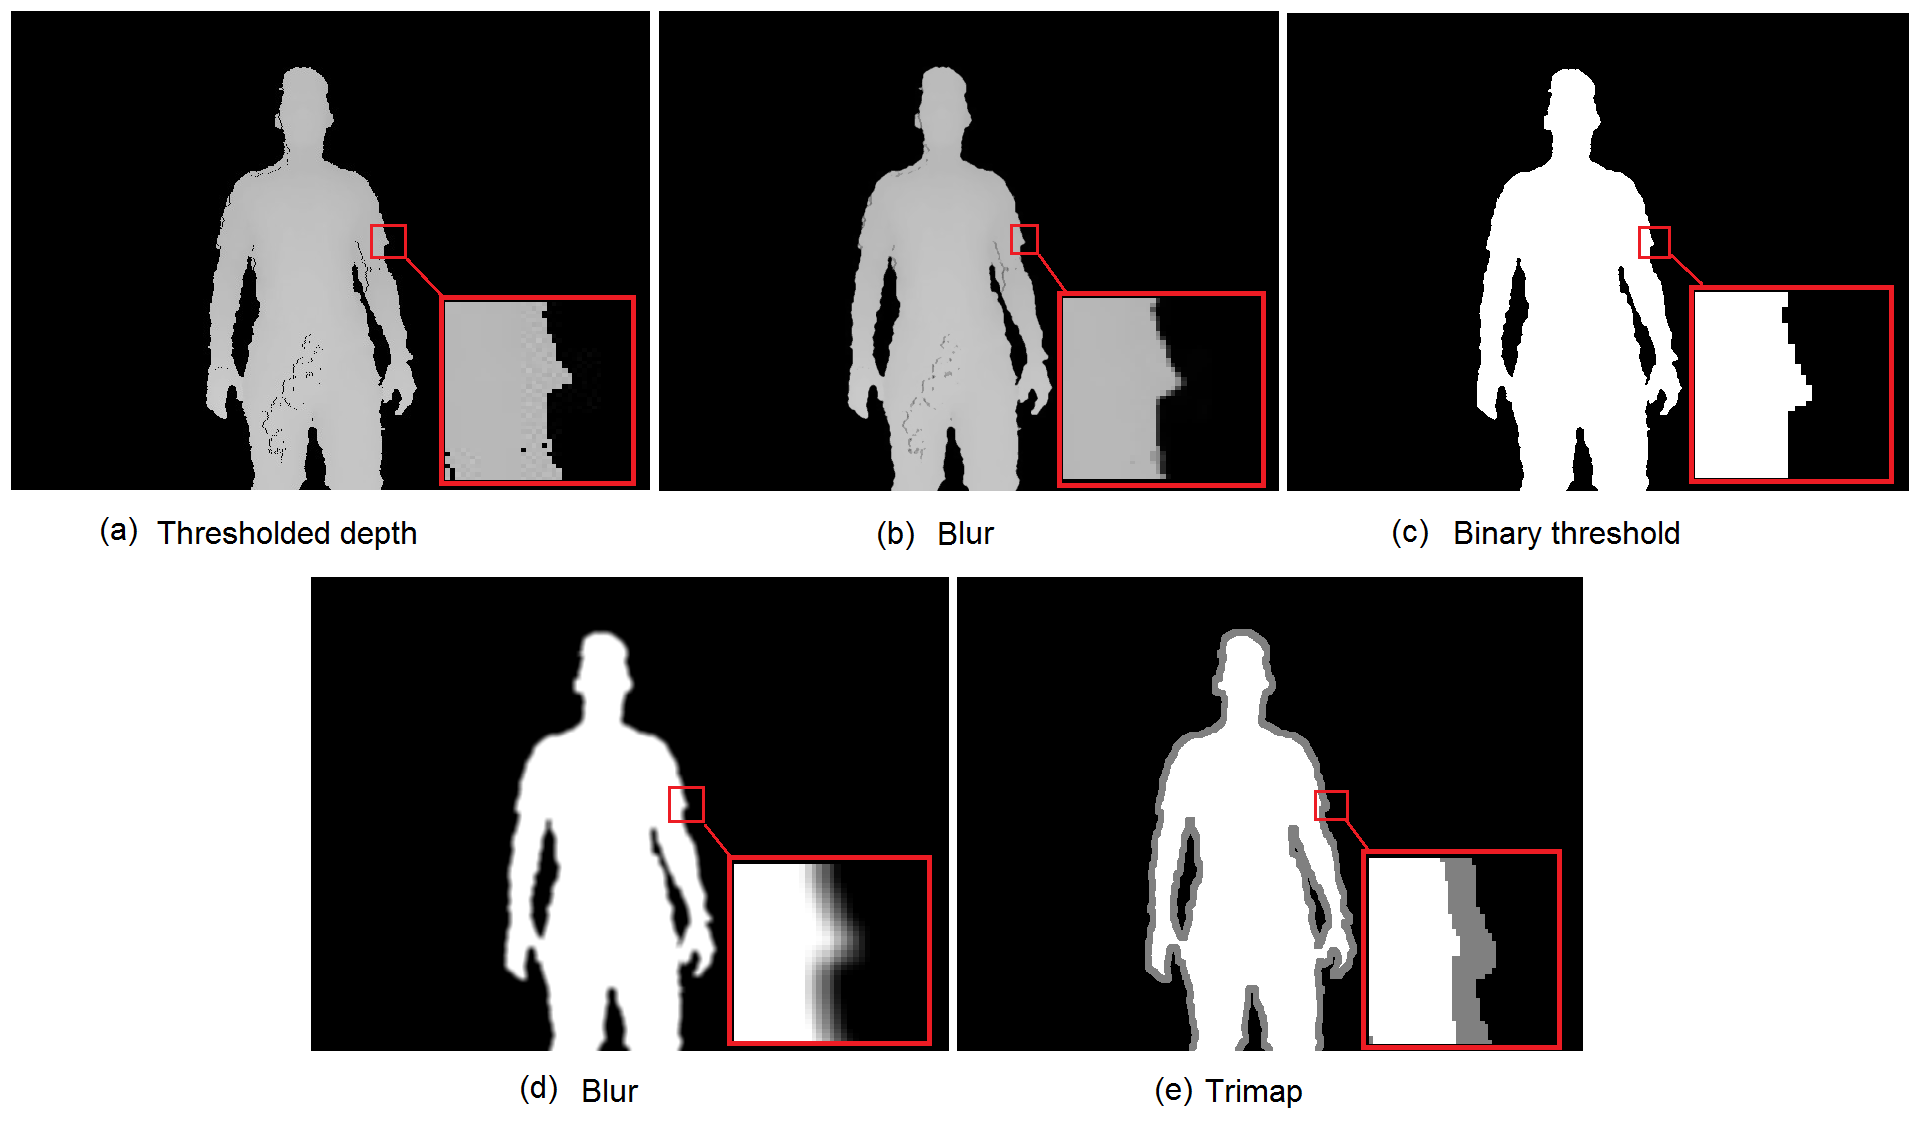
\includegraphics[width=1\columnwidth]{Chapter6/6/depth_work.png}
\caption[Work flow for trimap generation from depth.]{Work flow for trimap generation from depth.}
\label{fig:depth-work}
\end{figure}

%%%%%%%%%%%%%%%%%%%%%%%%%%%%%%%%%%%%%%%%%%%%%%%%%%%%%%%%%%%%%%%%%%%%%%%%%%%%%%%%%%%%%%%%%%%%%%
\section{Combining the matting algorithm with the automatically generated trimap}
\label{sec:combining-matting-algorithm-with-trimap}

The automatically generated trimap is then used along with our matting algorithm to compute an alpha matte. As mentioned previously, since the purpose of the application is to extract a human figure from the background and the fuzzy regions are limited, we are using a minimal number of samples to be gathered that correspond to the thin unknown region and keep running times low. For feature comparison in the classification part of the method we only use RGB values. For smoothness and noise reduction of the estimated alpha matte we use a median filter (Figure \ref{fig:post-work}).

\begin{figure}[t!]
\centering
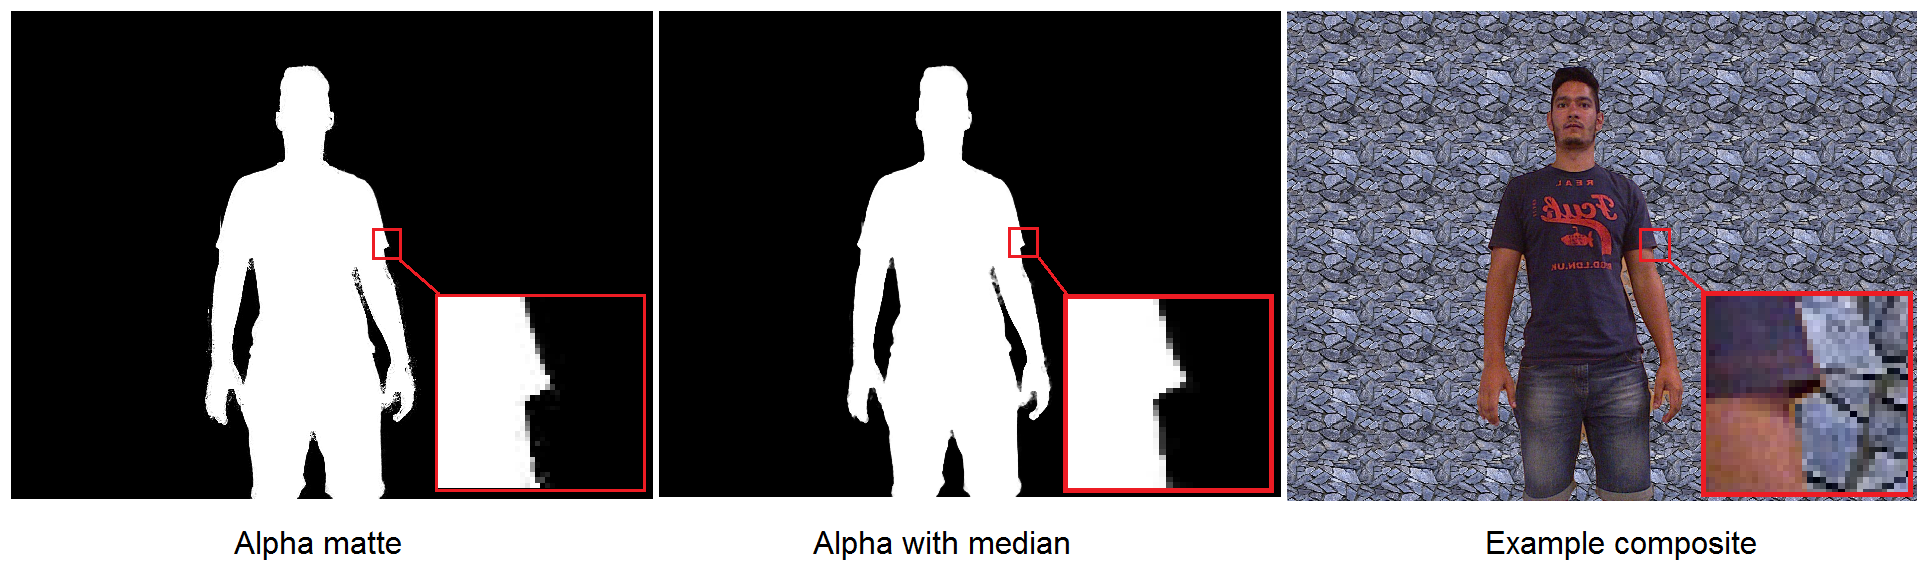
\includegraphics[width=1\columnwidth]{Chapter6/6/post_work.png}
\caption[Estimated alpha matte and an example composite.]{Estimated alpha matte and an example composite.}
\label{fig:post-work}
\end{figure}

\section{Results and comparisons}
\label{sec:comparisons-app}

Experimental results are compared using the the automatically generated trimap with the Kinect sensor, manually defined trimaps and comparison of results produced from running the Closed-Form algorithms on our images. The Closed-Form algorithm implementation was taken from the authors website. Running times for the whole process range from 1 to 5 seconds for a 640x480 image, depending on the size of the unknown region.
In all figures, results are based on images with moderate to difficult backgrounds, since images with an easy background are practically 100\% accurate.
\par
In Figure \ref{fig:res1-f}b and \ref{fig:res2-f}b a worst case scenario trimap is presented that could be the result of a scribble based used input. The use of such a wide trimap results in misclassification of many unknown pixels (Figure \ref{fig:res1-f}c \& \ref{fig:res2-f}c) and the Closed-Form algorithm due to its smoothness component erroneously adds additional foreground regions. Using a well defined trimap (Figure \ref{fig:res1-f}d \& \ref{fig:res2-f}d), the resulting alpha matte is almost 100\% accurate (Figure \label{fig:res1-f}e \& \ref{fig:res2-f}e), and in comparison with the automatically generated trimap (Figure \label{fig:res1-f}f \& \ref{fig:res2-f}f) the resulting alpha matte (Figure \ref{fig:res1-f}g \& \ref{fig:res2-f}g) is similar but has some regions that are wrong due to errors in the automatic trimap. These errors are due to noise in the depth-map that our method did not manage to remove. By widening the unknown region to compensate for the errors of the depth-map, results become similar to the ones in Figures \ref{fig:res1-f}c \& \ref{fig:res2-f}c.
\par
Figures \ref{fig:res1-f} and \ref{fig:res2-f} present results using high resolution images taken from the Kinect and by up-scalling the depth-map between lines 12-13 in Algorithm \ref{trimap-algorithm}. Similarly to the lower resolution images, when using a wide trimap many unknown pixels are miss-classified (Figure \ref{fig:res1-f}d \& \ref{fig:res2-f}d). The results from the use of the well defined trimaps are quite accurate (Figure \ref{fig:res3-f}f \& \ref{fig:res4-f}f) as in previous results, and the automatic trimap also produces visually acceptable results in-spite of having some miss-classified pixels that again are due to the fact that the depth-map has errors. In general high resolution images may have a more unknown pixels to classify but visually results are slightly better because the higher the resolution the more apparent the differences between regions.

\begin{figure}[t!]
%\centering
\subfloat[][RGB image]{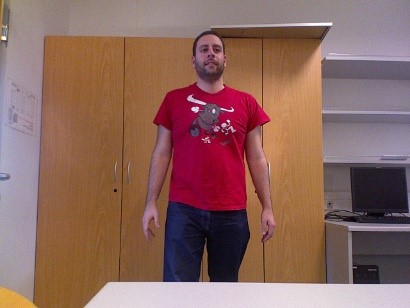
\includegraphics[width=0.5\columnwidth]{Chapter6/6/res1_color.png}}
\subfloat[][Wide trimap]{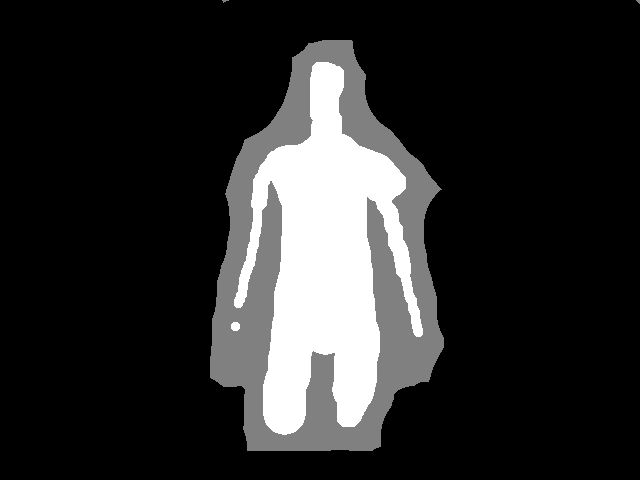
\includegraphics[width=0.5\columnwidth]{Chapter6/6/res1_wide_trimap.png}}
\newline
\subfloat[][Comparison of Closed-form and our result]{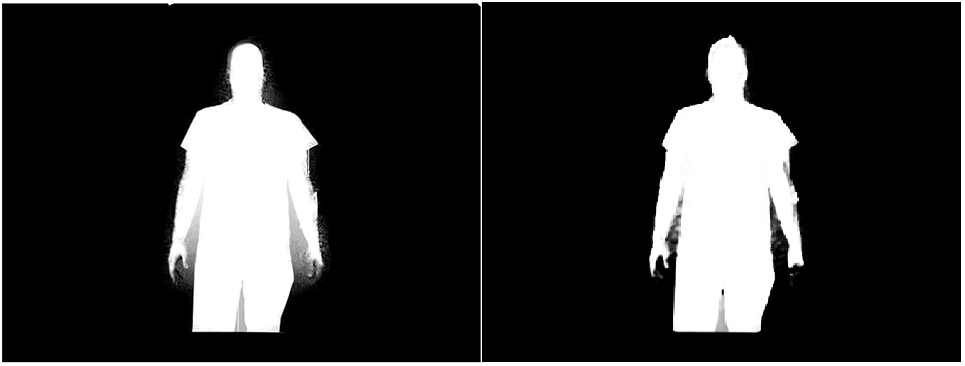
\includegraphics[width=1\columnwidth]{Chapter6/6/res1_wide.png}}
\newline
\subfloat[][Manual narrow trimap]{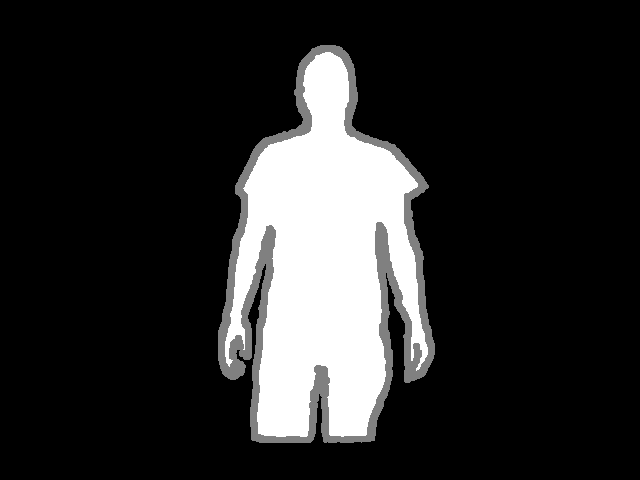
\includegraphics[width=0.5\columnwidth]{Chapter6/6/res1_narrow_trimap.png}}
\subfloat[][Result]{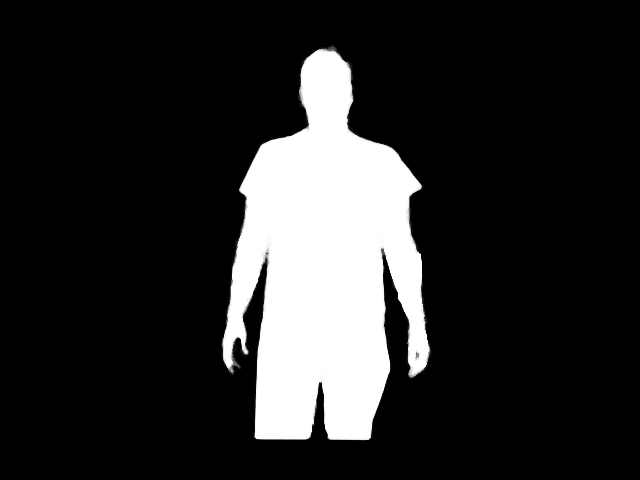
\includegraphics[width=0.5\columnwidth]{Chapter6/6/res1_manual.png}}
\newline
\subfloat[][Auto narrow trimap]{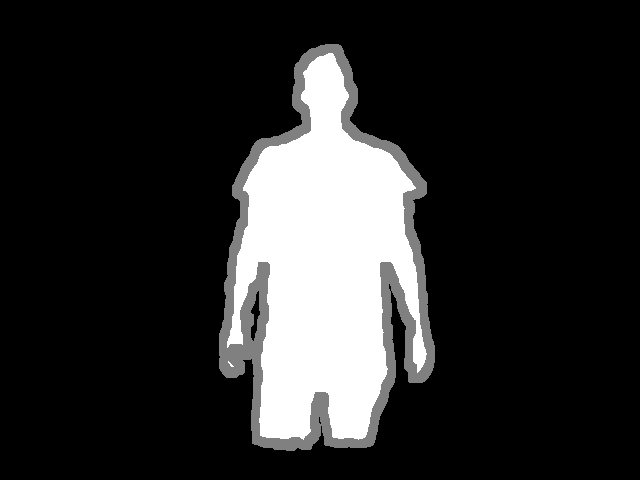
\includegraphics[width=0.5\columnwidth]{Chapter6/6/res1_auto_trimap.png}}
\subfloat[][Result]{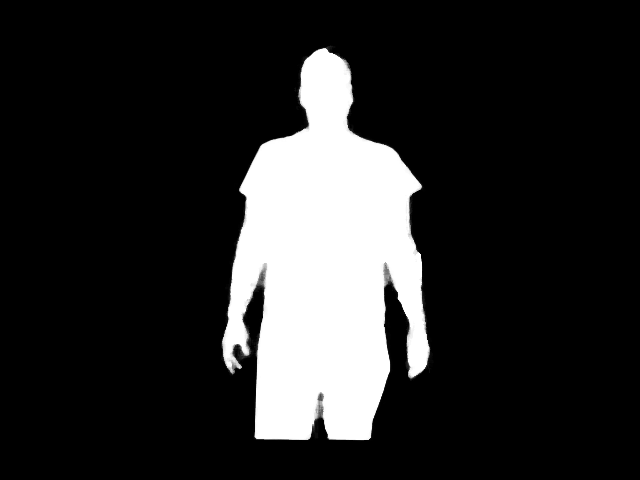
\includegraphics[width=0.5\columnwidth]{Chapter6/6/res1_auto.png}}
\caption[Trimaps and resulting alpha mattes.]{Trimaps and resulting alpha mattes.}
\label{fig:res1-f}
\end{figure}

\begin{figure}[t!]
%\centering
\subfloat[][RGB image]{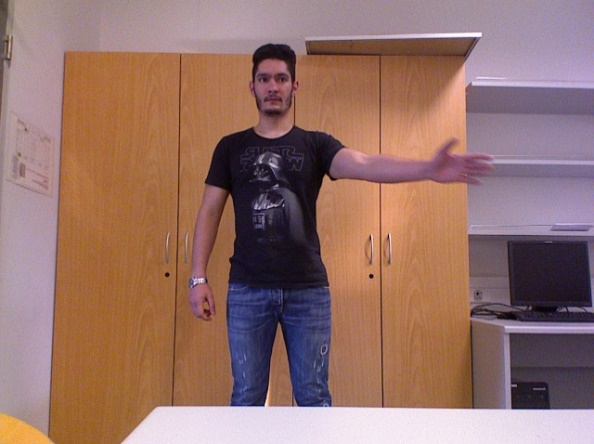
\includegraphics[width=0.5\columnwidth]{Chapter6/6/res2_color.png}}
\subfloat[][Wide trimap]{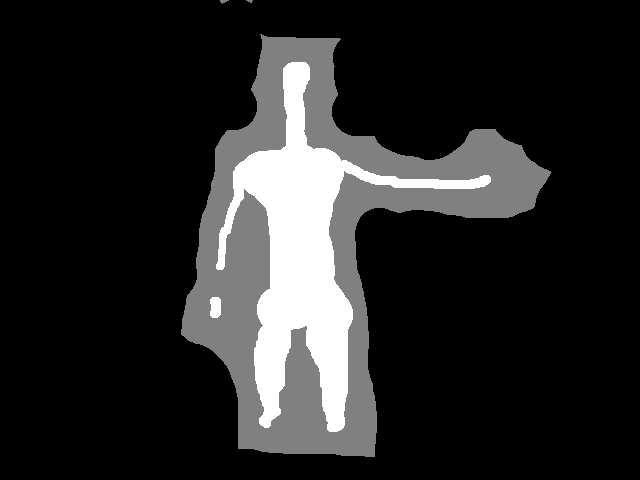
\includegraphics[width=0.5\columnwidth]{Chapter6/6/res2_wide_trimap.png}}
\newline
\subfloat[][Comparison of Closed-form and our result]{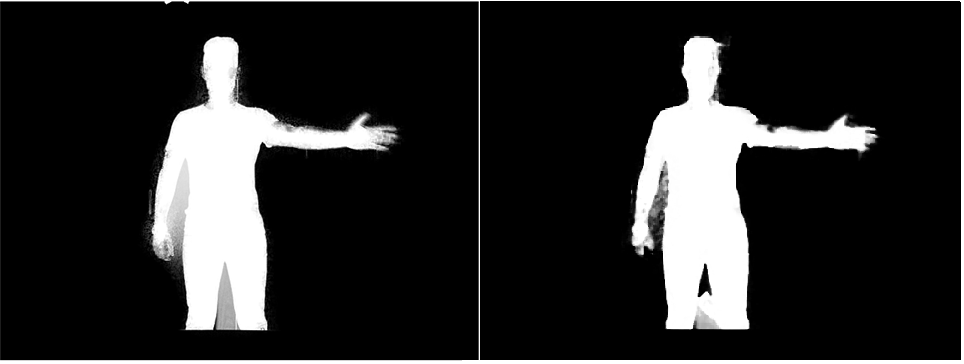
\includegraphics[width=1\columnwidth]{Chapter6/6/res2_wide.png}}
\newline
\subfloat[][Manual narrow trimap]{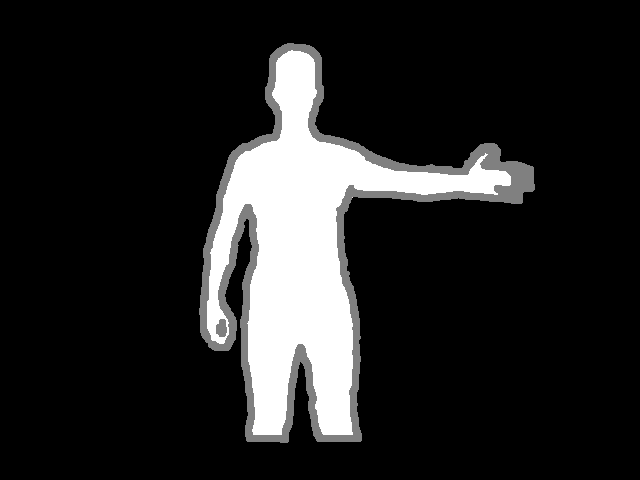
\includegraphics[width=0.5\columnwidth]{Chapter6/6/res2_narrow_trimap.png}}
\subfloat[][Result]{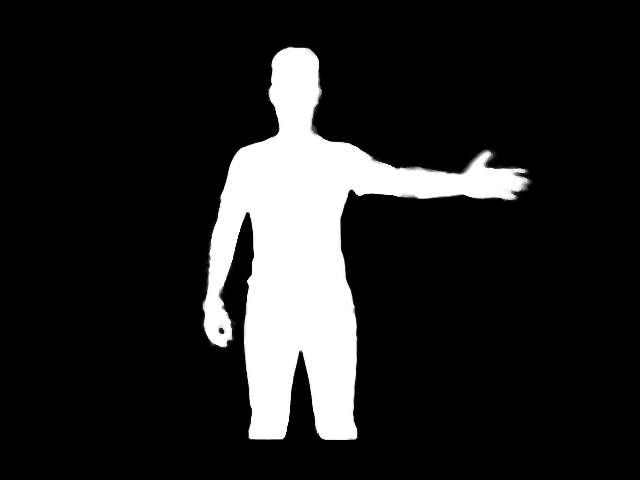
\includegraphics[width=0.5\columnwidth]{Chapter6/6/res2_manual.png}}
\newline
\subfloat[][Auto narrow trimap]{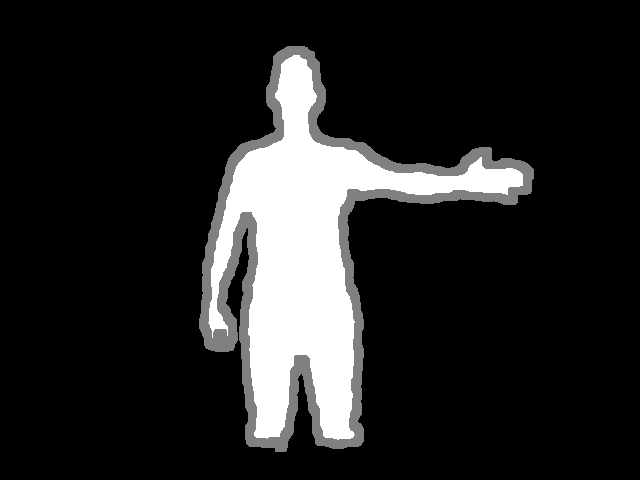
\includegraphics[width=0.5\columnwidth]{Chapter6/6/res2_auto_trimap.png}}
\subfloat[][Result]{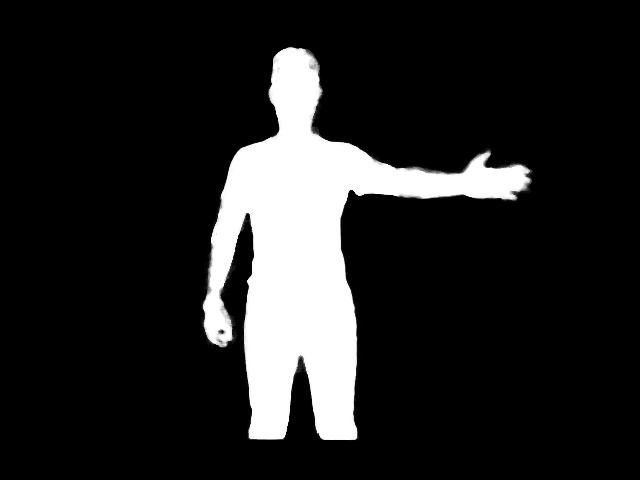
\includegraphics[width=0.5\columnwidth]{Chapter6/6/res2_auto.png}}
\caption[Trimaps and resulting alpha mattes.]{Trimaps and resulting alpha mattes.}
\label{fig:res2-f}
\end{figure}

\begin{figure}[t!]
%\centering
\subfloat[][RGB image]{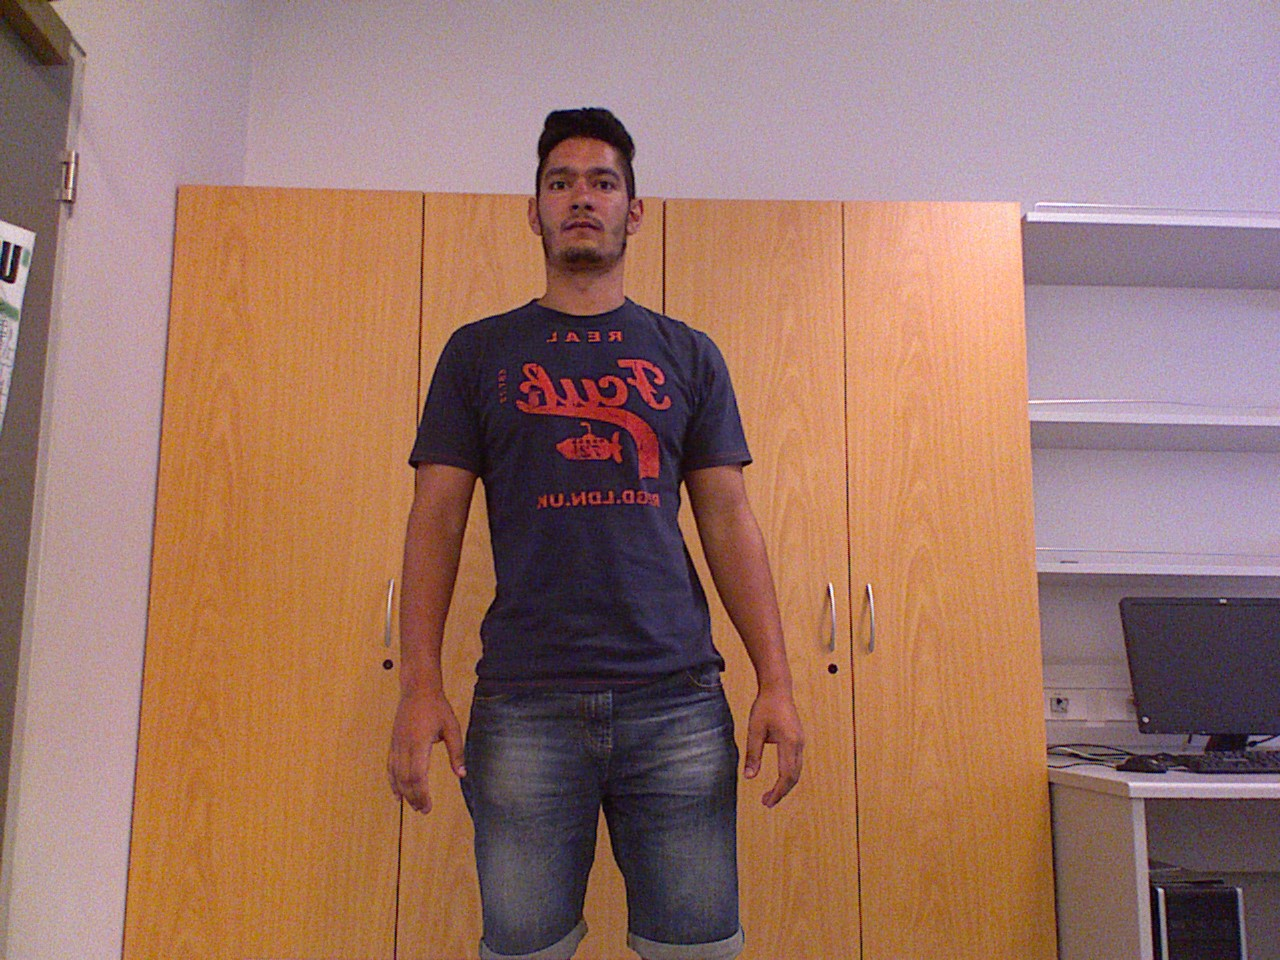
\includegraphics[width=0.5\columnwidth]{Chapter6/6/res3_color.png}}
\subfloat[][Thresholded depth-map]{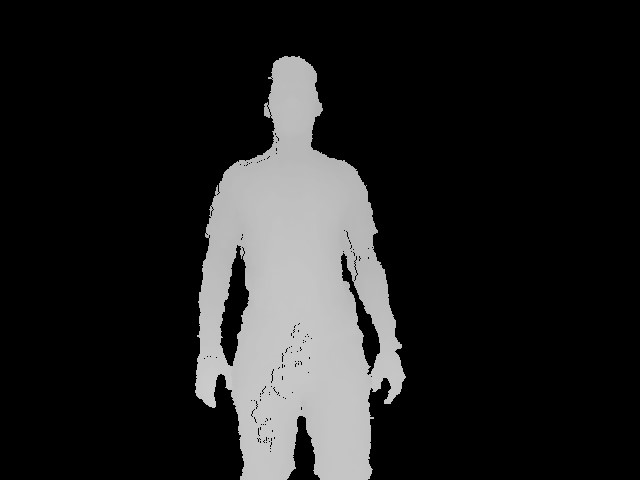
\includegraphics[width=0.5\columnwidth]{Chapter6/6/res3_depth.png}}
\newline
\subfloat[][Wide trimap]{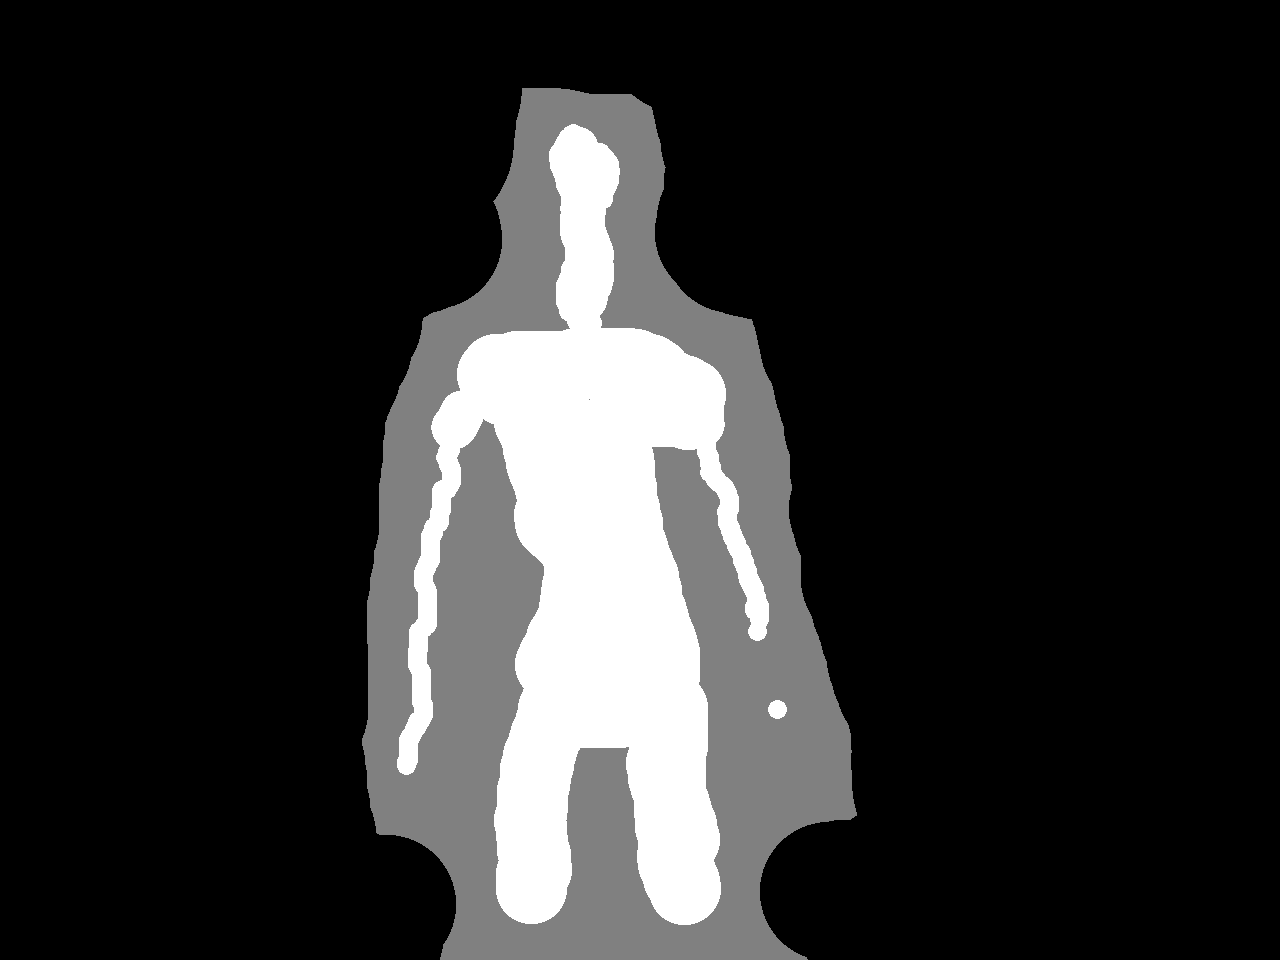
\includegraphics[width=0.5\columnwidth]{Chapter6/6/res3_wide_trimap.png}}
\subfloat[][Result]{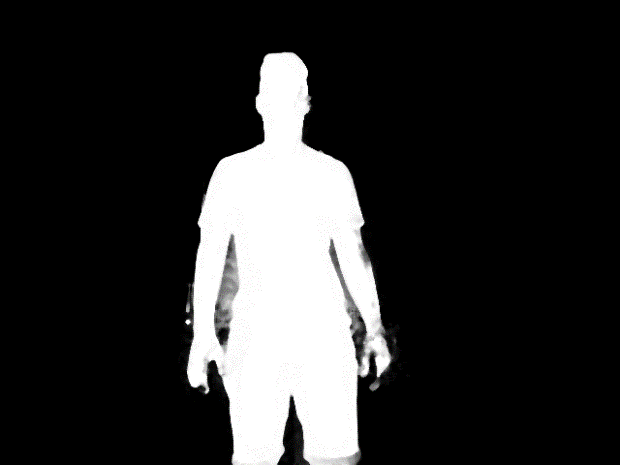
\includegraphics[width=0.5\columnwidth]{Chapter6/6/res3_wide.png}}
\newline
\subfloat[][Manual narrow trimap]{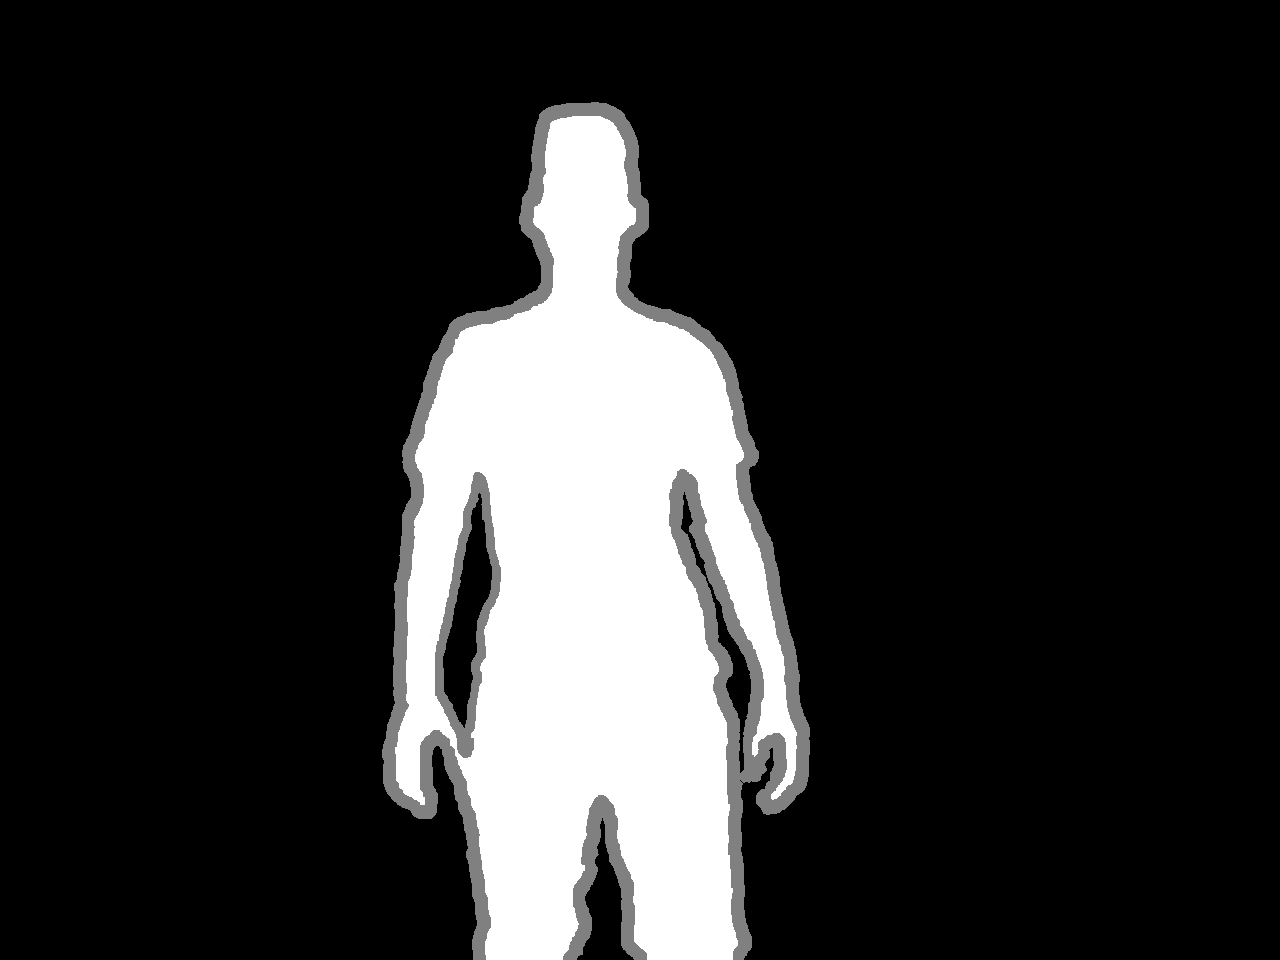
\includegraphics[width=0.5\columnwidth]{Chapter6/6/res3_manual_trimap.png}}
\subfloat[][Result]{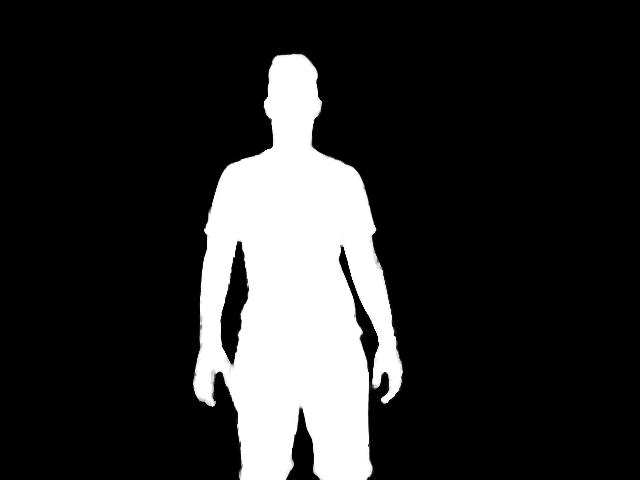
\includegraphics[width=0.5\columnwidth]{Chapter6/6/res3_manual.png}}
\newline
\subfloat[][Auto narrow trimap]{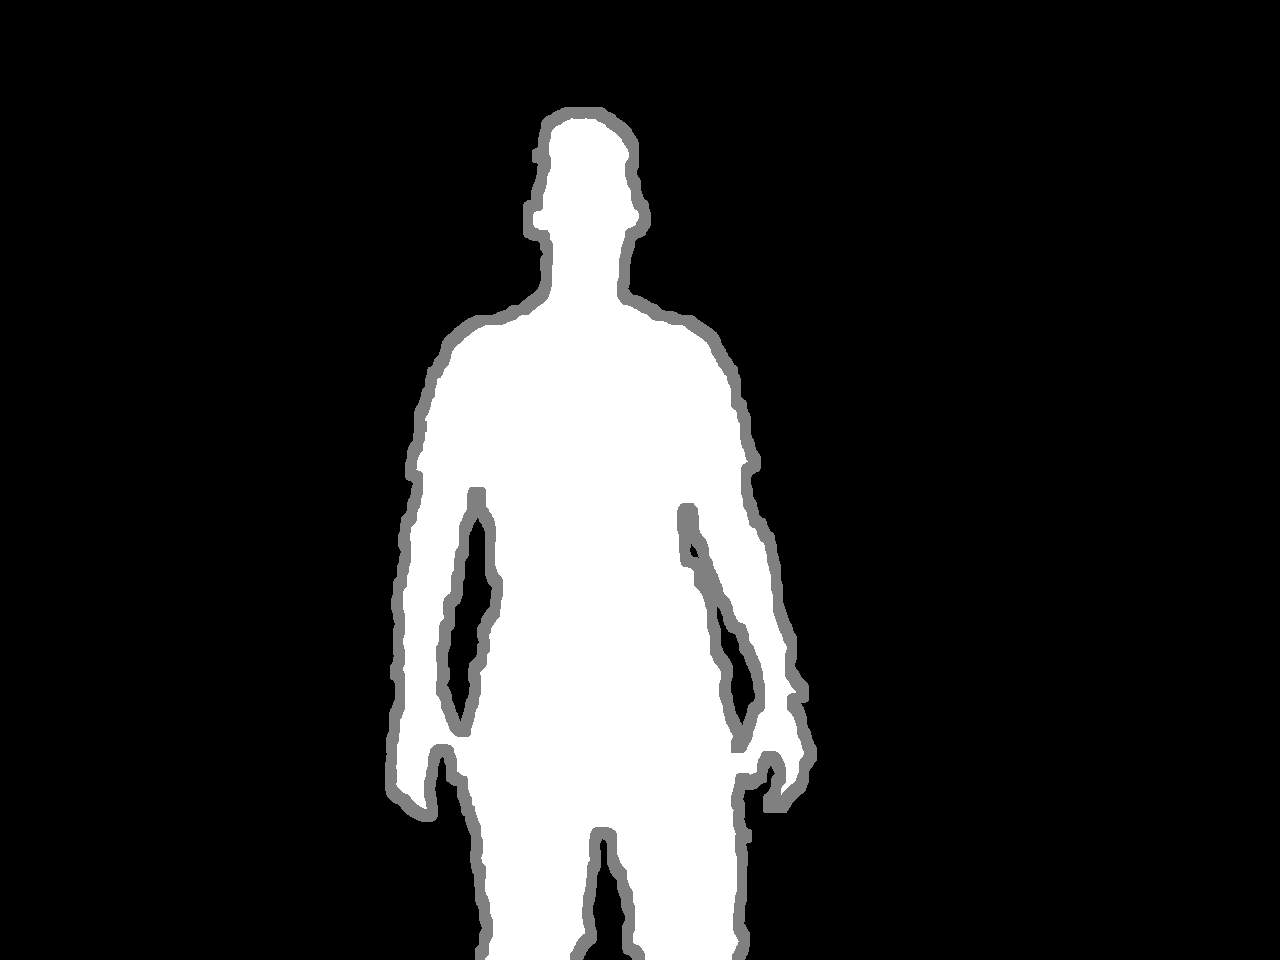
\includegraphics[width=0.5\columnwidth]{Chapter6/6/res3_auto_trimap.png}}
\subfloat[][Result]{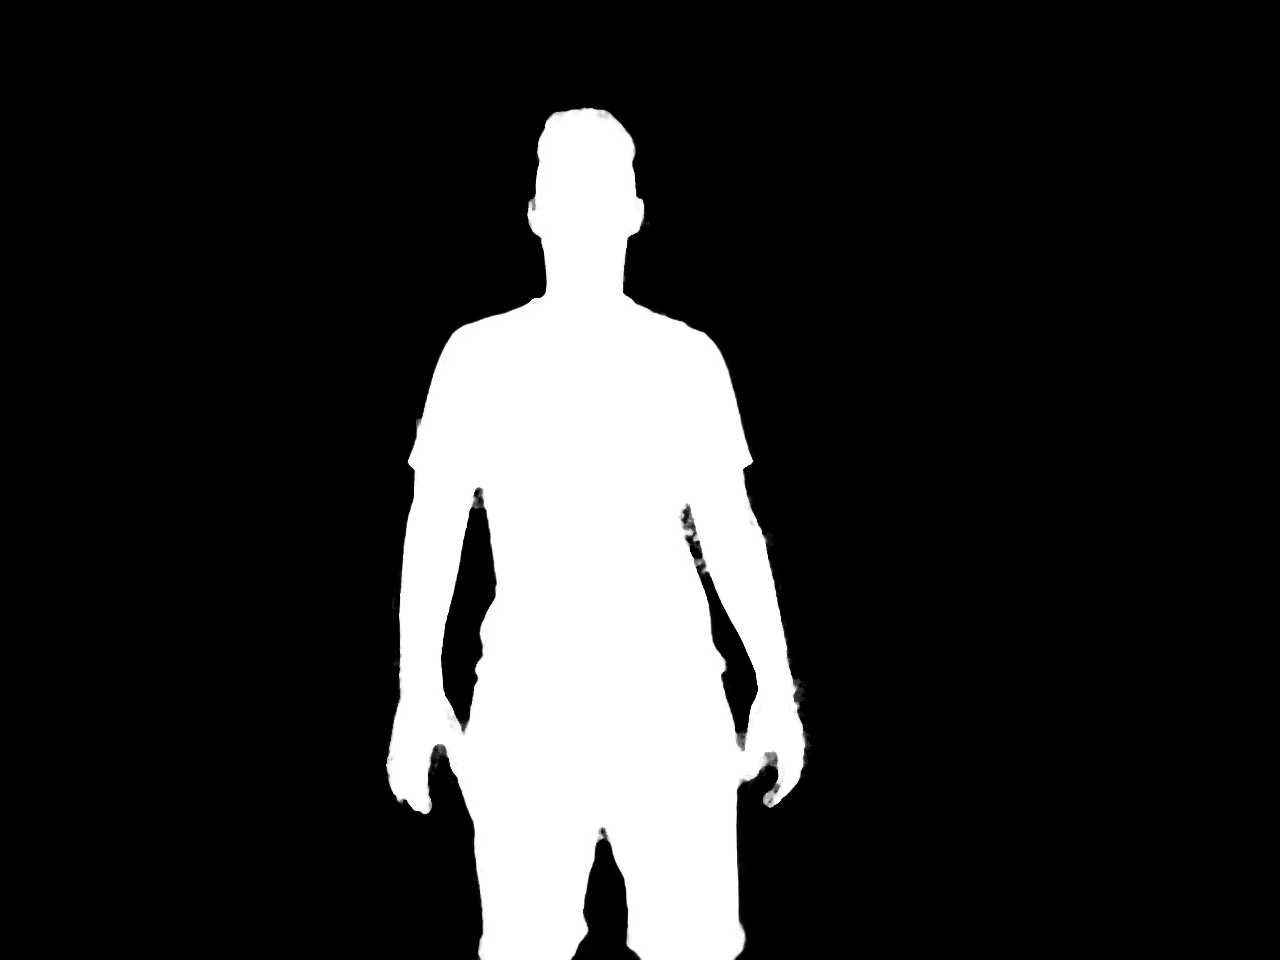
\includegraphics[width=0.5\columnwidth]{Chapter6/6/res3_auto.png}}
\caption[Trimaps and resulting alpha mattes.]{Trimaps and resulting alpha mattes.}
\label{fig:res3-f}
\end{figure}

\begin{figure}[t!]
%\centering
\subfloat[][RGB image]{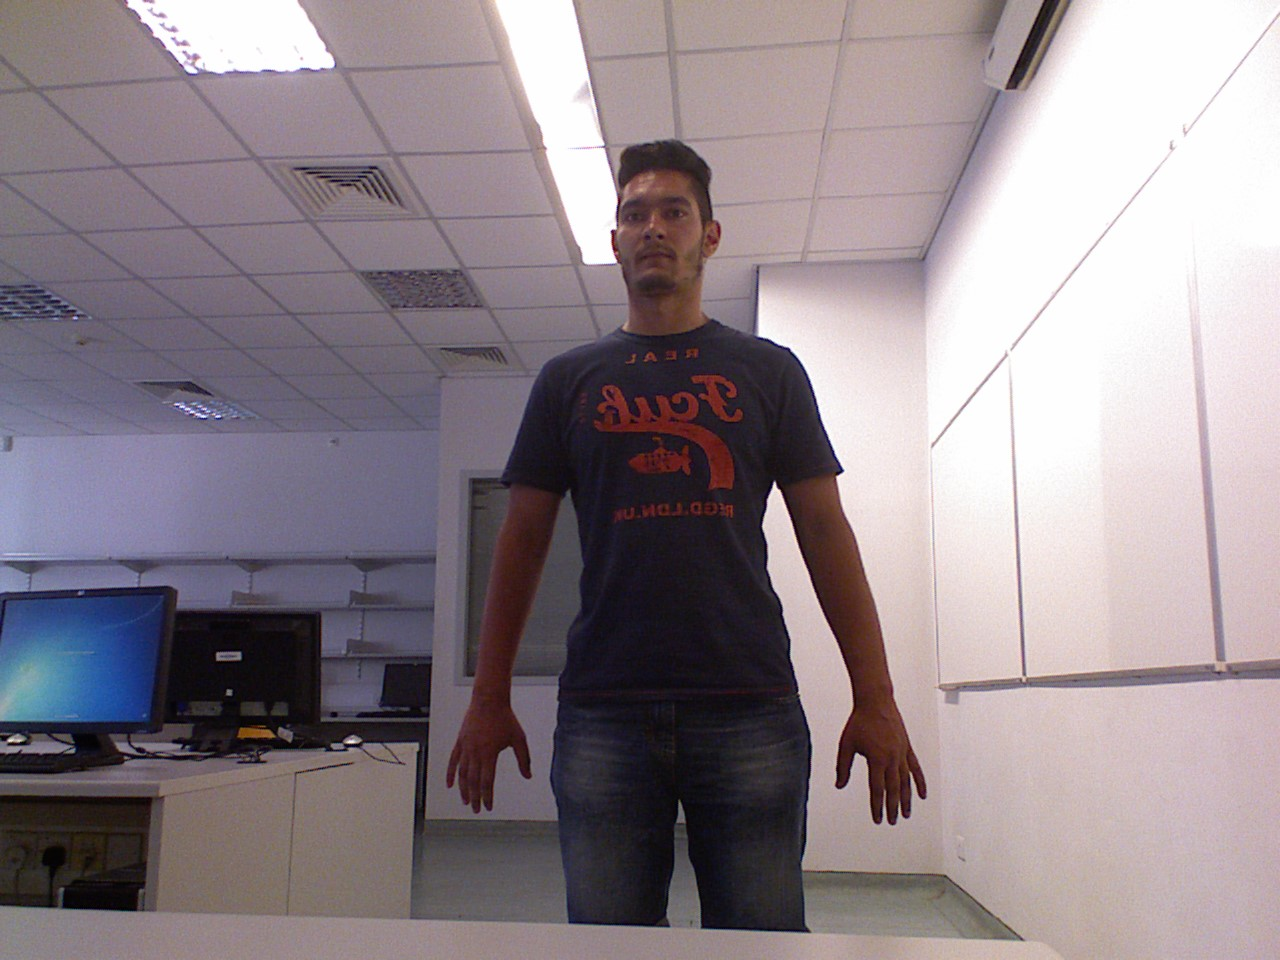
\includegraphics[width=0.5\columnwidth]{Chapter6/6/res4_color.png}}
\subfloat[][Thresholded depth-map]{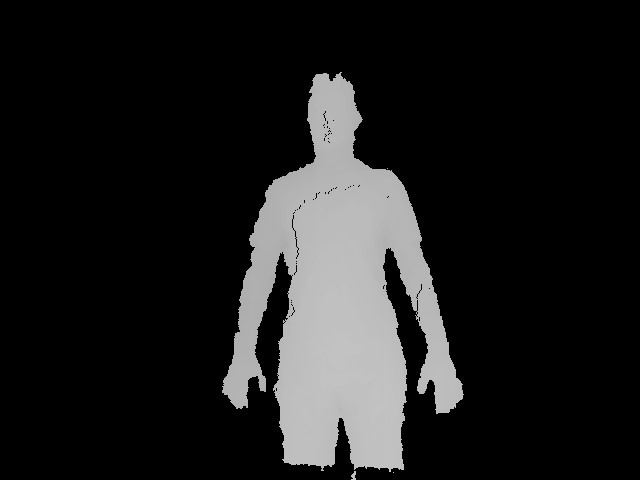
\includegraphics[width=0.5\columnwidth]{Chapter6/6/res4_depth.png}}
\newline
\subfloat[][Wide trimap]{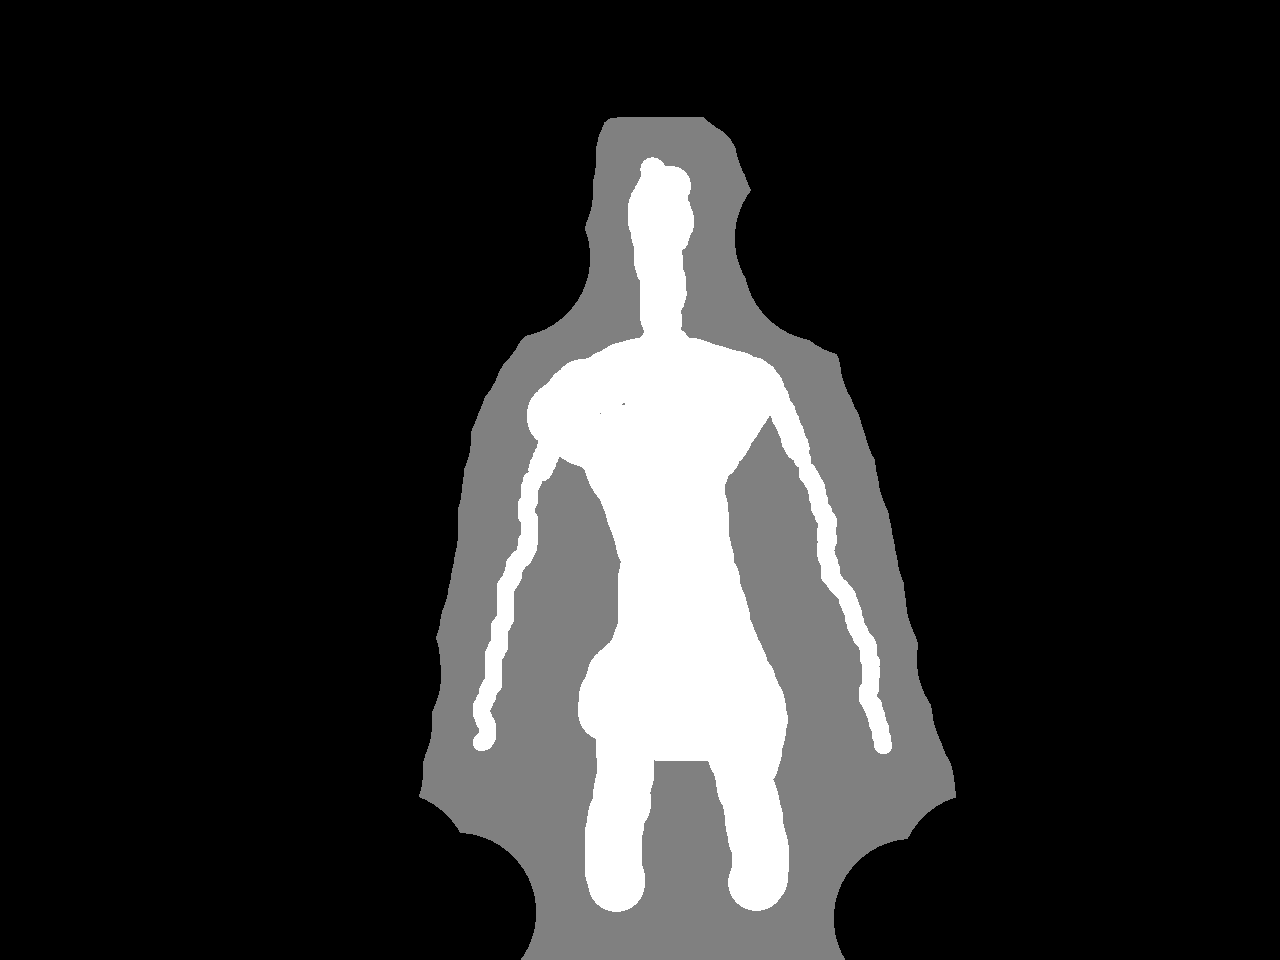
\includegraphics[width=0.5\columnwidth]{Chapter6/6/res4_wide_trimap.png}}
\subfloat[][Result]{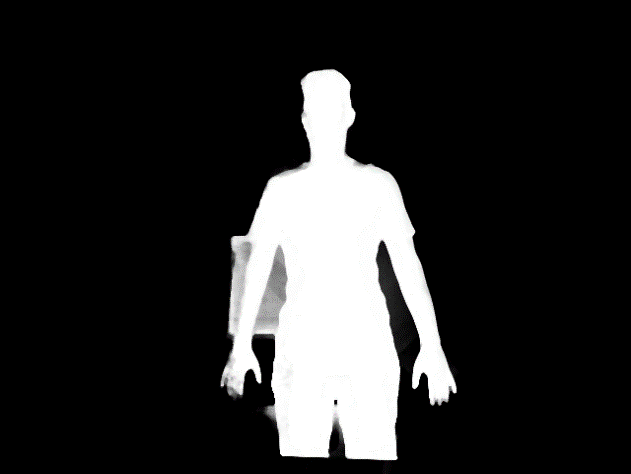
\includegraphics[width=0.5\columnwidth]{Chapter6/6/res4_wide.png}}
\newline
\subfloat[][Manual narrow trimap]{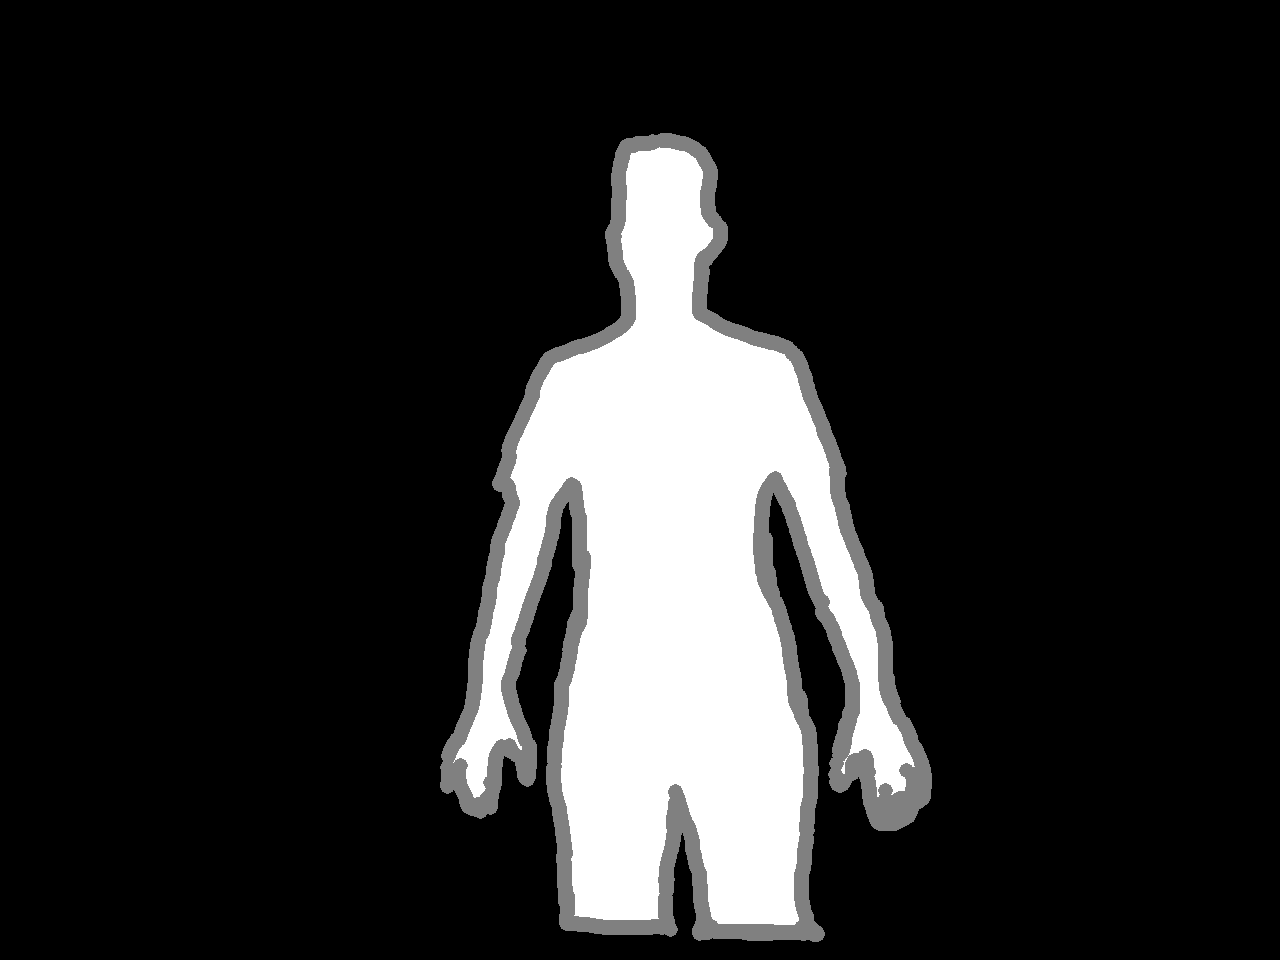
\includegraphics[width=0.5\columnwidth]{Chapter6/6/res4_manual_trimap.png}}
\subfloat[][Result]{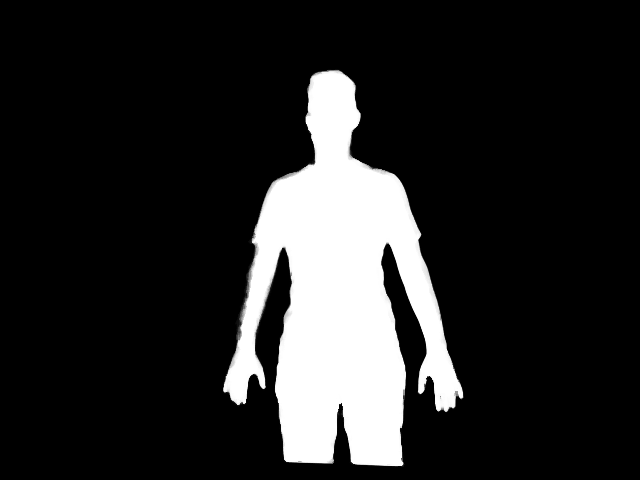
\includegraphics[width=0.5\columnwidth]{Chapter6/6/res4_manual.png}}
\newline
\subfloat[][Auto narrow trimap]{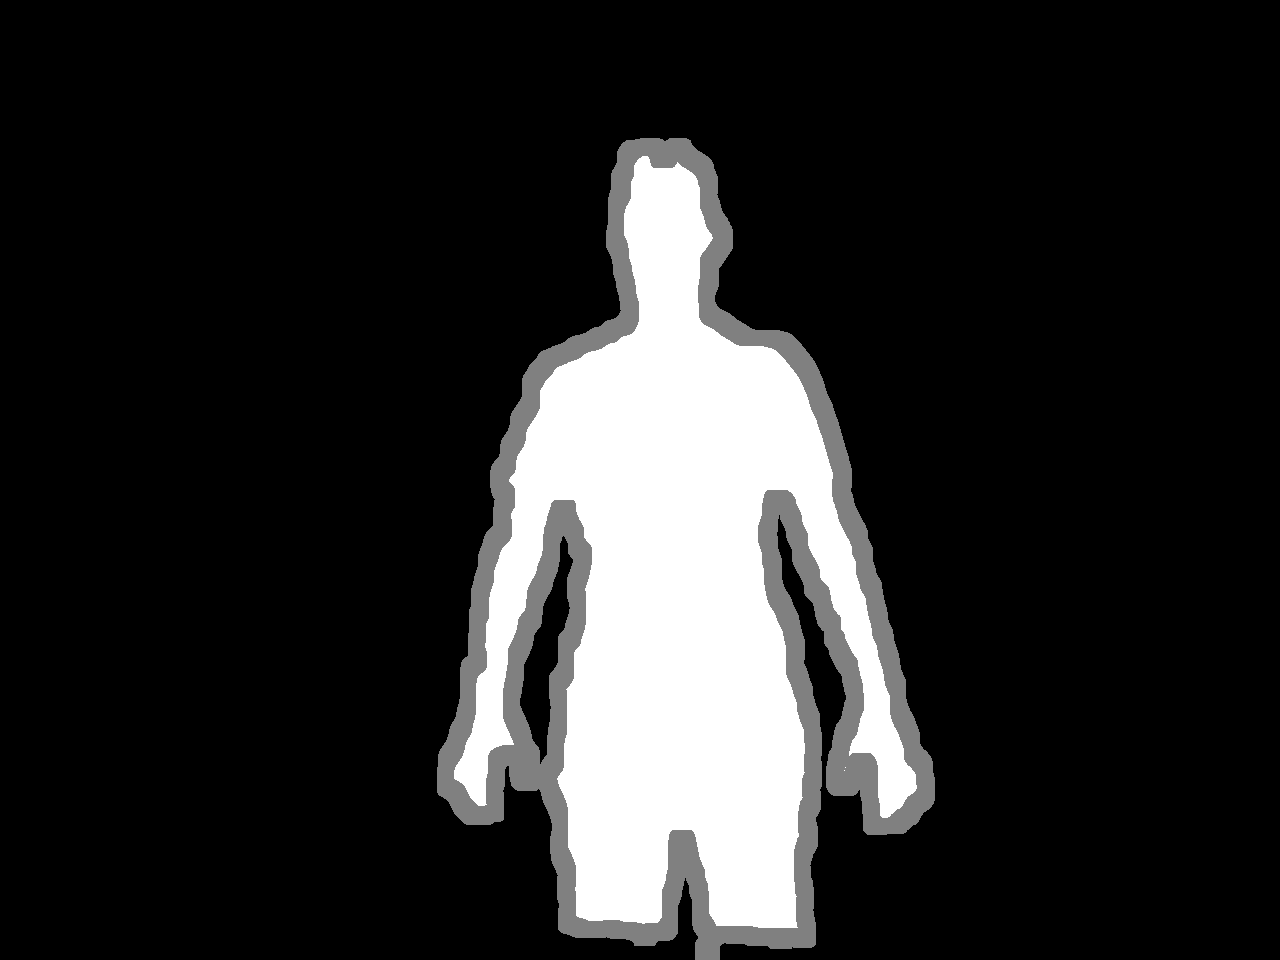
\includegraphics[width=0.5\columnwidth]{Chapter6/6/res4_auto_trimap.png}}
\subfloat[][Result]{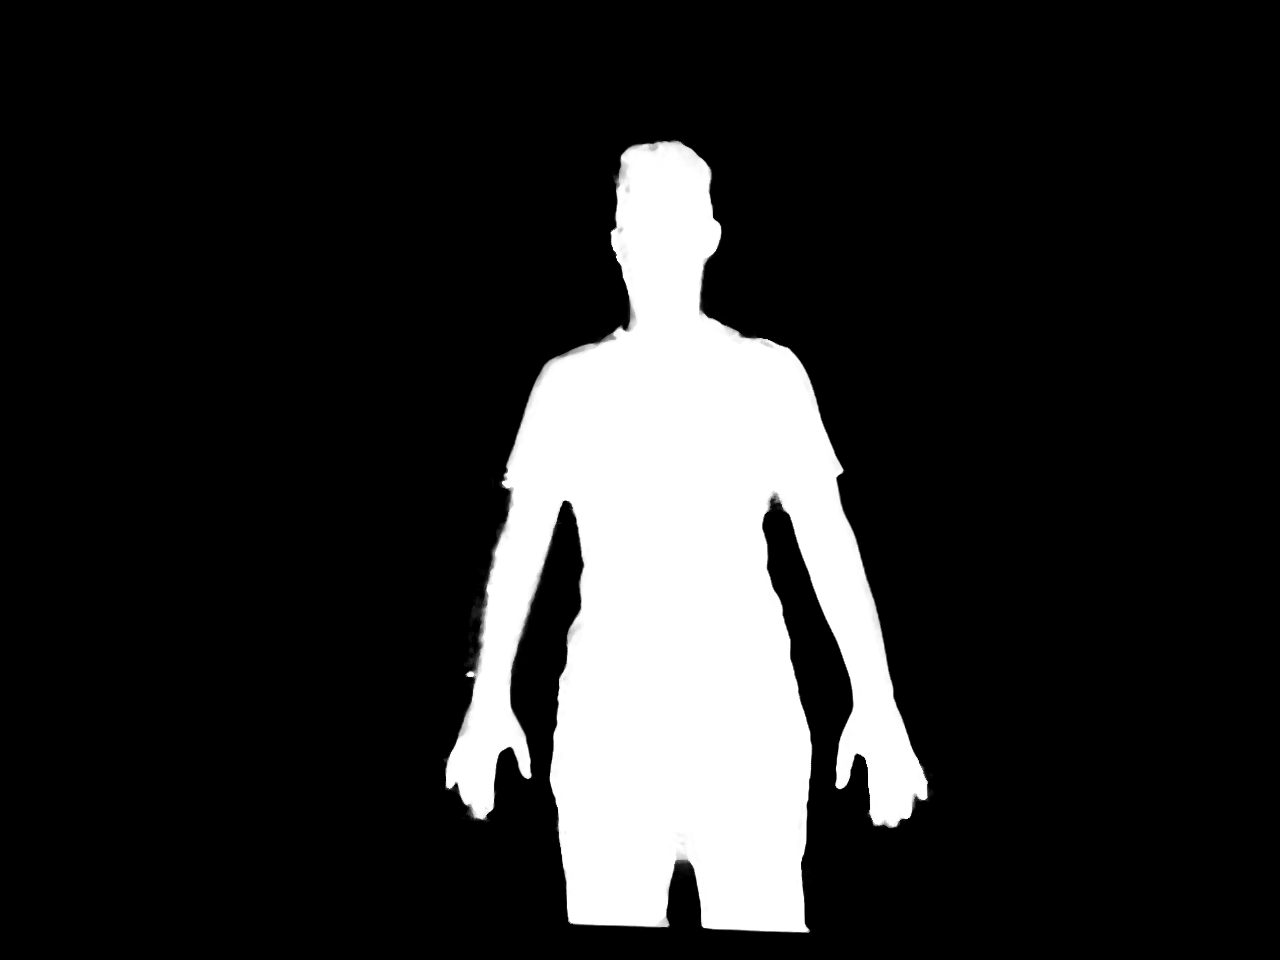
\includegraphics[width=0.5\columnwidth]{Chapter6/6/res4_auto.png}}
\caption[Trimaps and resulting alpha mattes.]{Trimaps and resulting alpha mattes.}
\label{fig:res4-f}
\end{figure}


